% You should title the file with a .tex extension (hw1.tex, for example)
\documentclass[11pt]{article}

\usepackage{hyperref}
\usepackage{amsmath}
\usepackage{mathtools}
\usepackage{amssymb}
\usepackage{wrapfig}
\usepackage{fancyhdr}
\usepackage{tikz-qtree}
\usepackage{tikz-qtree-compat}
\usepackage[normalem]{ulem}
\usepackage{tikz}
\usepackage{graphicx}
\DeclareMathOperator*{\argmin}{argmin}
\DeclareMathOperator*{\argmax}{argmax}

\oddsidemargin0cm
\topmargin-2cm     %I recommend adding these three lines to increase the 
\textwidth16.5cm   %amount of usable space on the page (and save trees)
\textheight23.5cm  

\newcommand{\question}[2] {\vspace{.25in} \hrule\vspace{0.5em}
\noindent{\bf #1: #2} \vspace{0.5em}
\hrule \vspace{.10in}}
\renewcommand{\part}[1] {\vspace{.10in} {\bf (#1)}}

\newcommand{\myname}{Sean Bittner}
\newcommand{\myandrew}{srb2201@columbia.edu}
\newcommand{\myhwnum}{12}

\setlength{\parindent}{0pt}
\setlength{\parskip}{5pt plus 1pt}
 
\DeclarePairedDelimiter\abs{\lvert}{\rvert}%
 %
\pagestyle{fancyplain}
\rhead{\fancyplain{}{\myname\\ \myandrew}}

\begin{document}

\medskip                        % Skip a "medium" amount of space
                                % (latex determines what medium is)
                                % Also try: \bigskip, \littleskip

\thispagestyle{plain}
\begin{center}                  % Center the following lines
{\Large STG introductory example} \\
Sean Bittner \\
May 22, 2019 \\
\end{center}

\section{Background}
As we've discussed, our introductory example for the DSN is going to be the STG.  We want to pick out the regions of conductance space that produce medium levels of hub neuron frequency 0.525Hz +- 0.025Hz (green, Fig. 2, Gutierrez et al. 2013). \\
\begin{center}
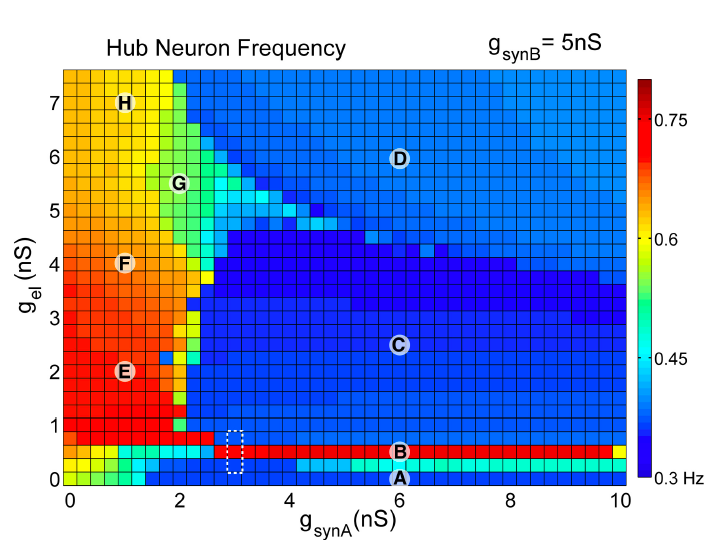
\includegraphics[scale=0.3]{figs/Gutierrez2013_Fig2.png}
\end{center}
Before training DSNs at the full resolution necessary to exactly reproduce this (T=800), I am using T=200 to get an idea of the appropriate augmented lagrangian optimization paramterization that will yield bio-modal (the two green areas below) distributions in this STG setting.
\begin{center}
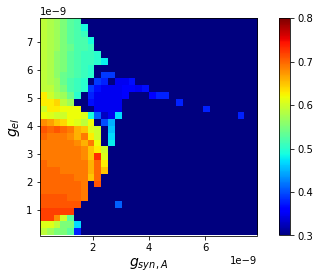
\includegraphics[scale=0.8]{DSN_figs/STG_T=200.png}
\end{center}

I ran 8 30-hour DSN training processes: $c_0 = 1, 100$ with 4 random initial seeds each.  Each 10 planar flow $\rightarrow$ scale $\rightarrow$ shift normalizing flow architecture was initialized to a truncated gaussian with mean of (4 nS, 4 nS), with a standard deviation of 3 nS.  Each augmented lagrangian epoch is 10,000 iterations.  This number of iterations for an augmented lagrangian epoch is much higher than I usually use, since we want to get close to convergence for by the end of each epoch.  This is desireable, since we want to reason about the dynamics of the entire AL optimization.  I am using an AL factor of $\beta = 4$ as in the MEFN paper, although we can modify this.

\section{Results}
\begin{center}
{\Large $c_0 = 1$} \\
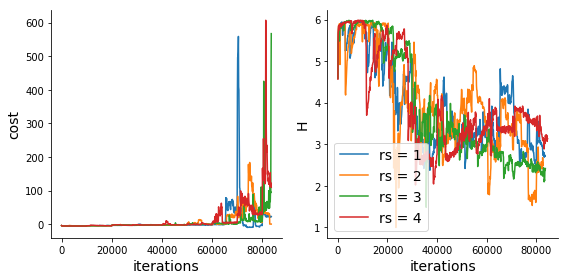
\includegraphics[scale=0.4]{DSN_figs/STG_DSN_c=0_H.png}
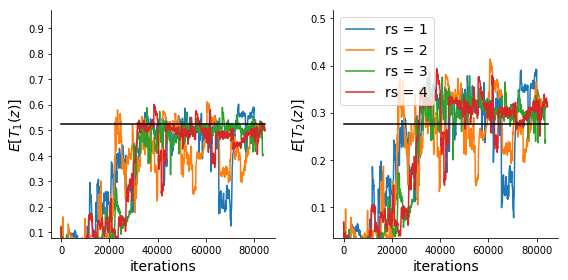
\includegraphics[scale=0.4]{DSN_figs/STG_DSN_c=0_cons.png} 
\end{center}
In each of the four optimizations, the entropy (H) initially increases, and begins to decrease during the 3-4th AL epoch.  At the beginning of the 2nd and 3rd AL epochs ($k=2, 3$), we should expect a relatively expansive distribution over the interval (0,20), (0, 20).  This is indeed what we see below, as we visualize the DSN distribution for each random seed at the beginning of each AL epoch.  

By the end of 8 AL epochs, none of the DSNs have converged via the hypothesis testing criteria, but they are rather close.  In general, the means are a bit too low, and the second moments are a bit too high.  (If the means are undershot and second moments are overshot, there is a considerably greater amount of variance in these plots then we will have at convergence.)  We see a mixture of DSNs which are still emitting samples in both green modes (rs = 1,4), and have focused on the upper, more expansive mode (rs = 2, 3).

\begin{center}
{\Large $c_0 = 1$, random seed = 1} \\
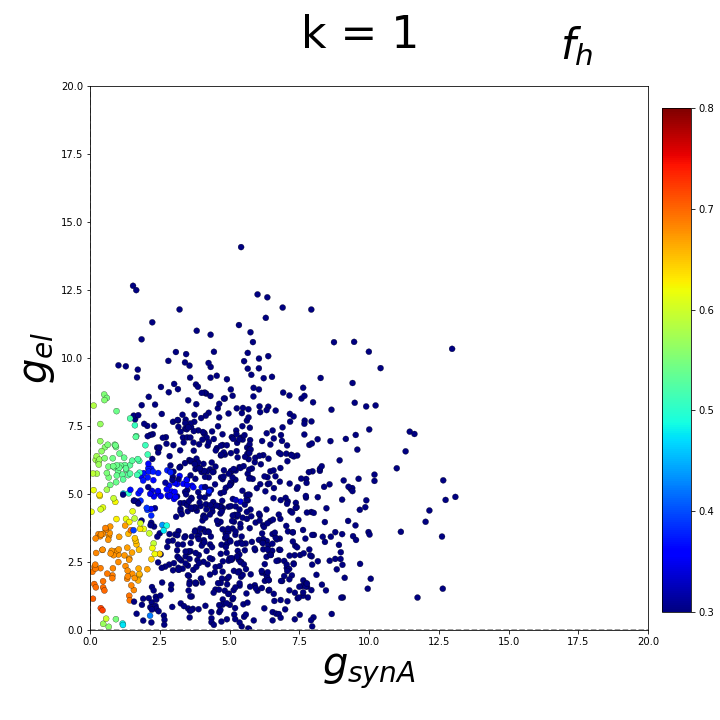
\includegraphics[scale=0.125]{DSN_figs/STGCircuit_DSN_c=0_rs=1_k=1.png}
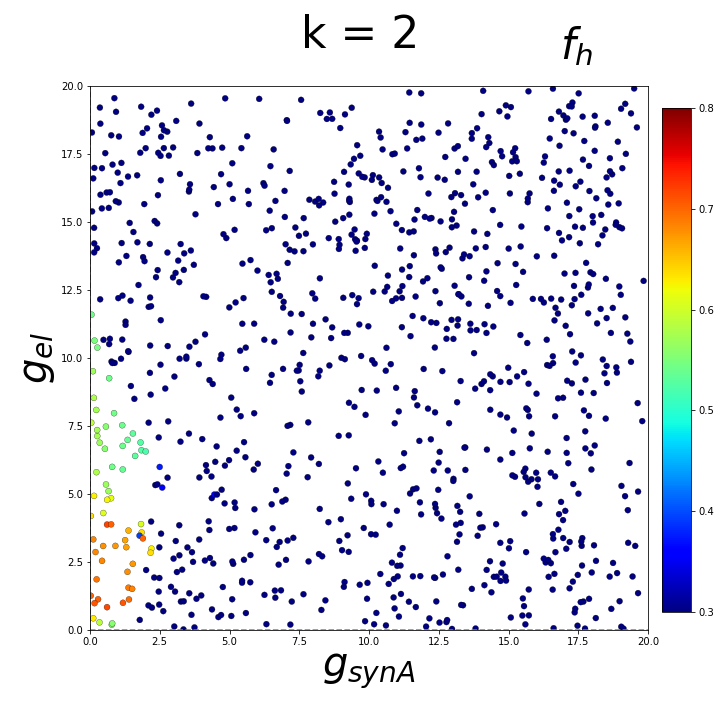
\includegraphics[scale=0.125]{DSN_figs/STGCircuit_DSN_c=0_rs=1_k=2.png}
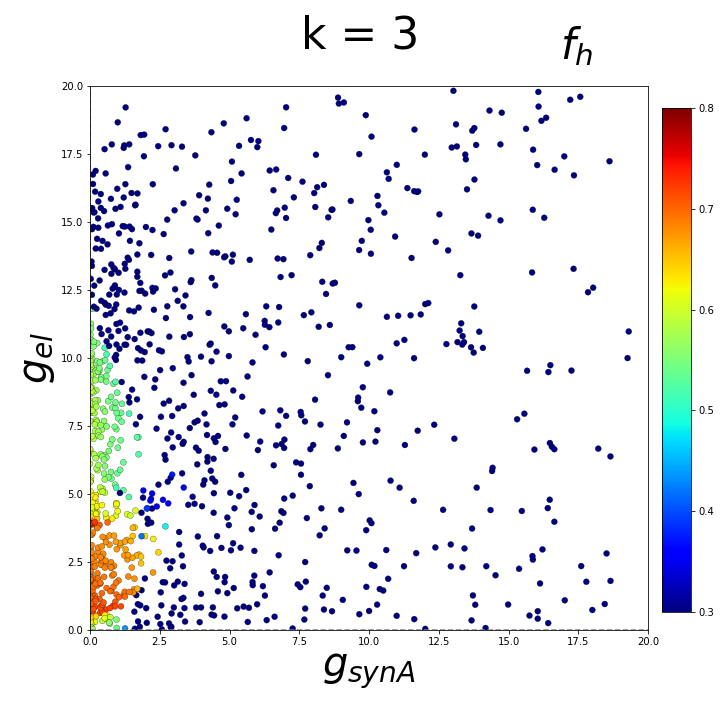
\includegraphics[scale=0.125]{DSN_figs/STGCircuit_DSN_c=0_rs=1_k=3.png}
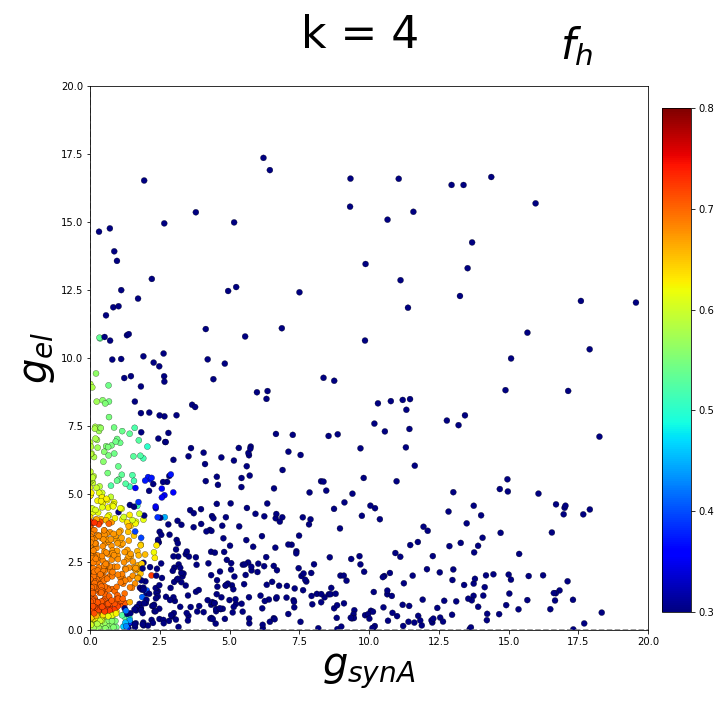
\includegraphics[scale=0.125]{DSN_figs/STGCircuit_DSN_c=0_rs=1_k=4.png}
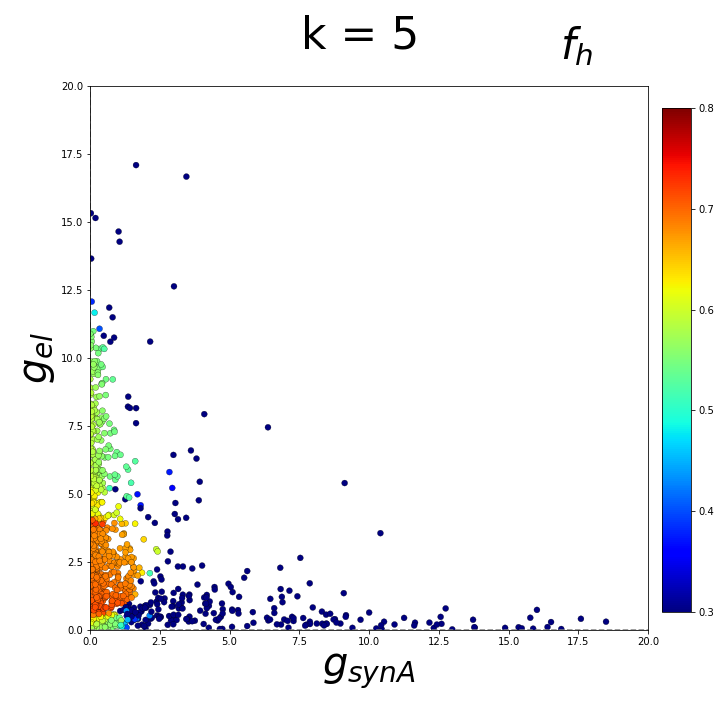
\includegraphics[scale=0.125]{DSN_figs/STGCircuit_DSN_c=0_rs=1_k=5.png}
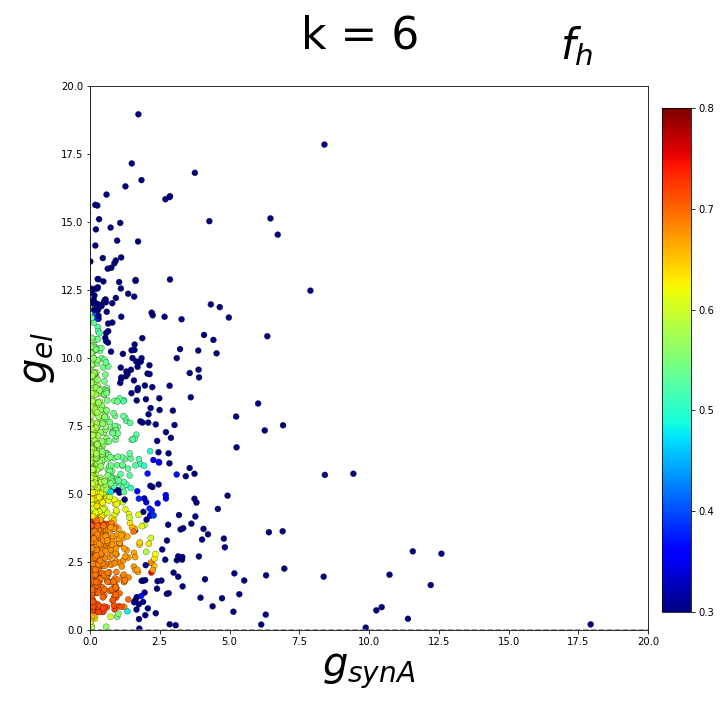
\includegraphics[scale=0.125]{DSN_figs/STGCircuit_DSN_c=0_rs=1_k=6.png}
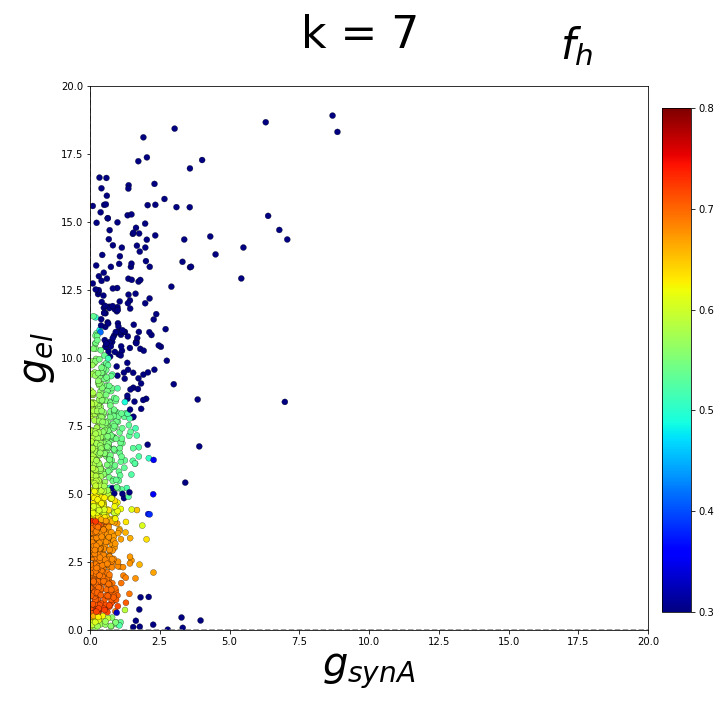
\includegraphics[scale=0.125]{DSN_figs/STGCircuit_DSN_c=0_rs=1_k=7.png}
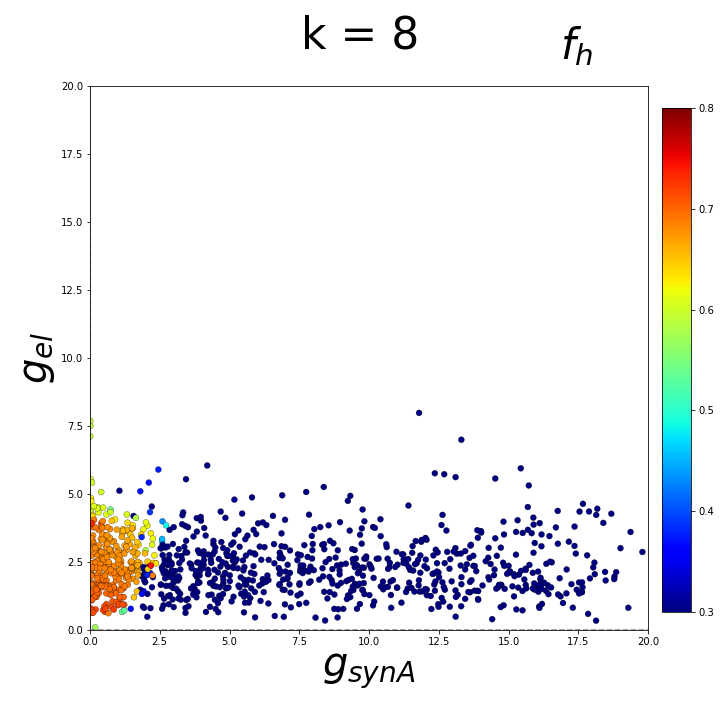
\includegraphics[scale=0.125]{DSN_figs/STGCircuit_DSN_c=0_rs=1_k=8.png}
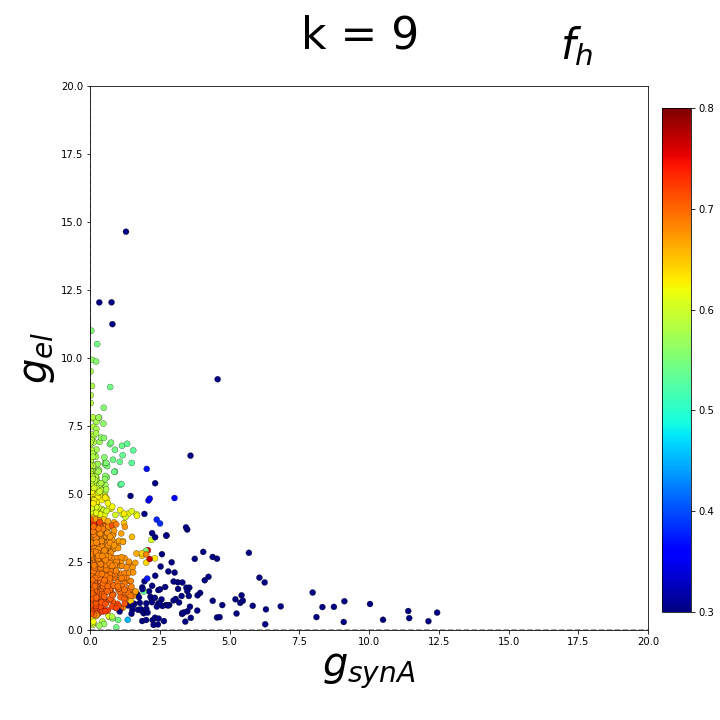
\includegraphics[scale=0.125]{DSN_figs/STGCircuit_DSN_c=0_rs=1_k=9.png}
\end{center}

\begin{center}
{\Large $c_0 = 1$, random seed = 2} \\
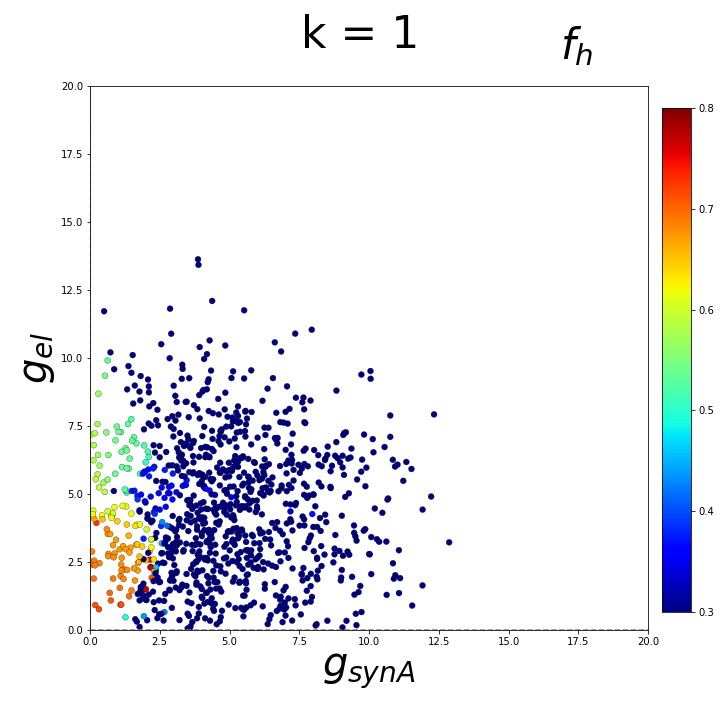
\includegraphics[scale=0.125]{DSN_figs/STGCircuit_DSN_c=0_rs=2_k=1.png}
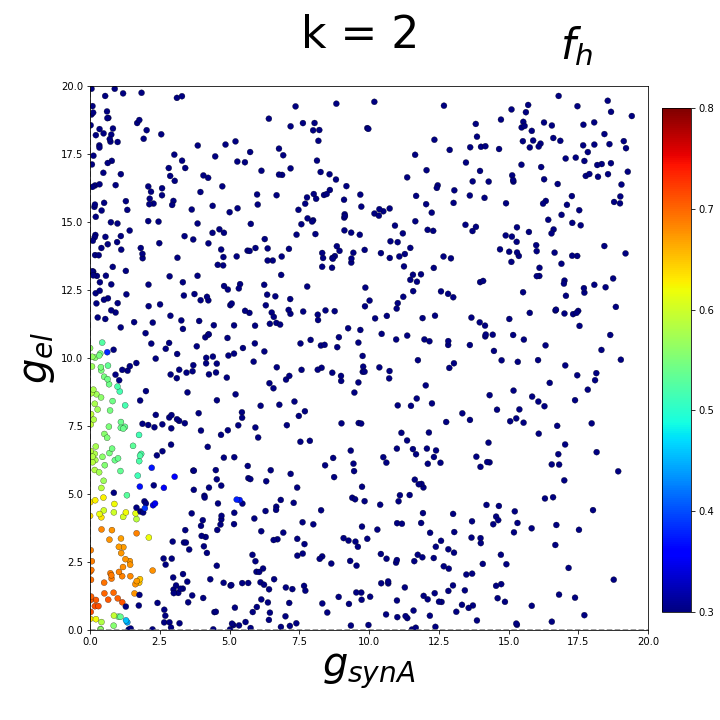
\includegraphics[scale=0.125]{DSN_figs/STGCircuit_DSN_c=0_rs=2_k=2.png}
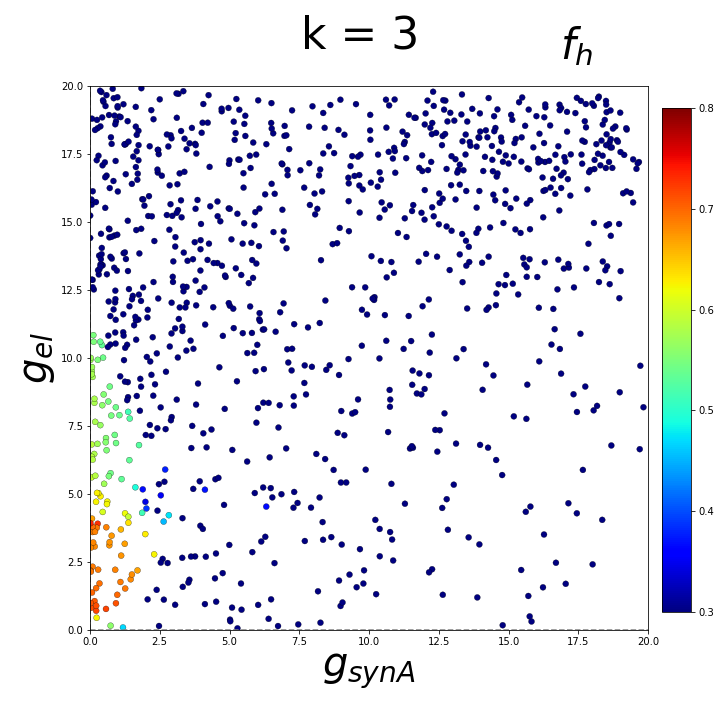
\includegraphics[scale=0.125]{DSN_figs/STGCircuit_DSN_c=0_rs=2_k=3.png}
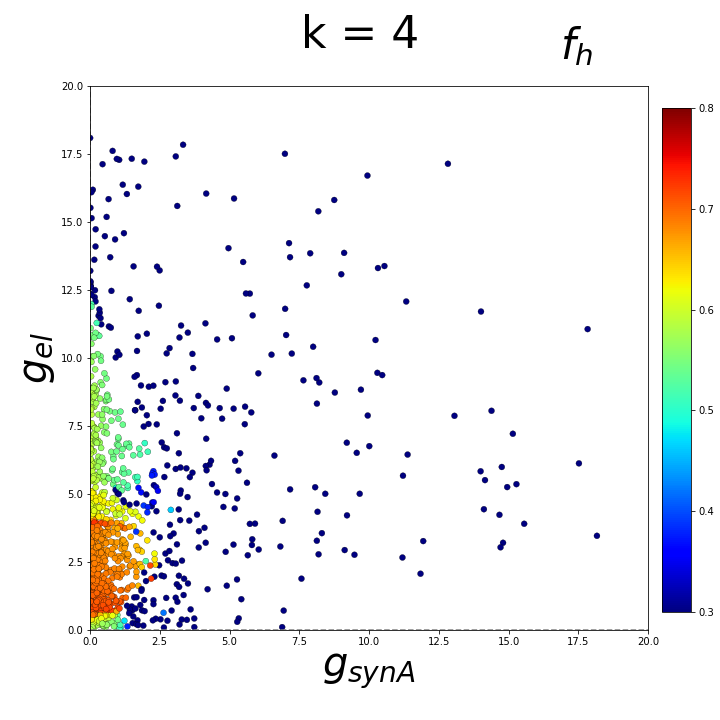
\includegraphics[scale=0.125]{DSN_figs/STGCircuit_DSN_c=0_rs=2_k=4.png}
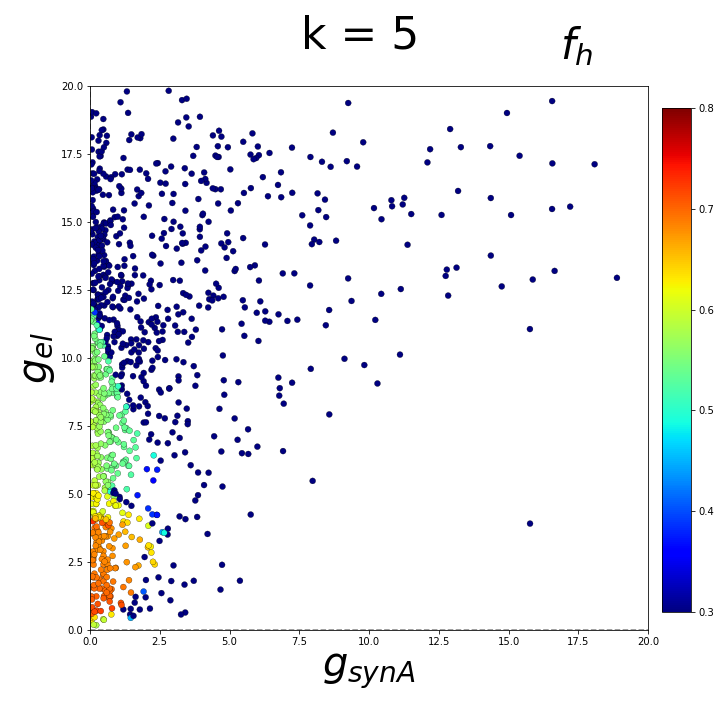
\includegraphics[scale=0.125]{DSN_figs/STGCircuit_DSN_c=0_rs=2_k=5.png}
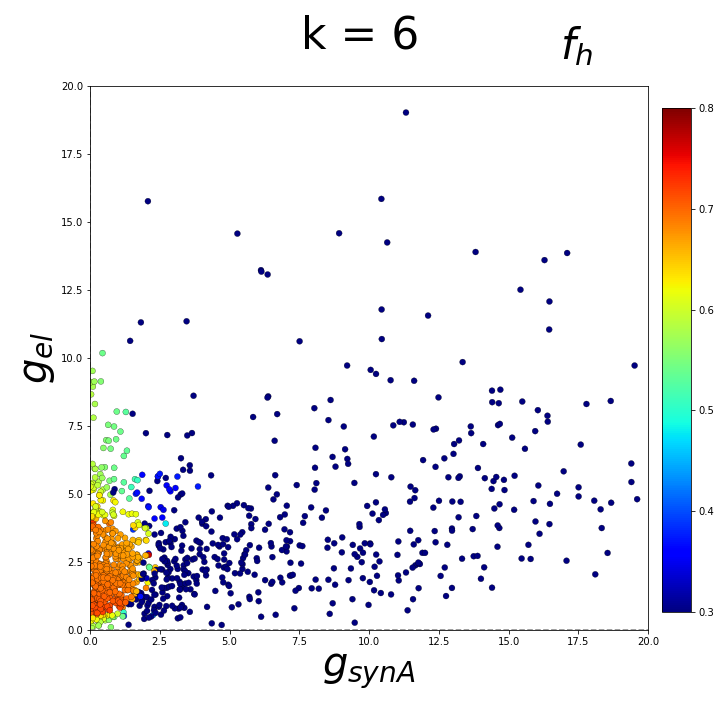
\includegraphics[scale=0.125]{DSN_figs/STGCircuit_DSN_c=0_rs=2_k=6.png}
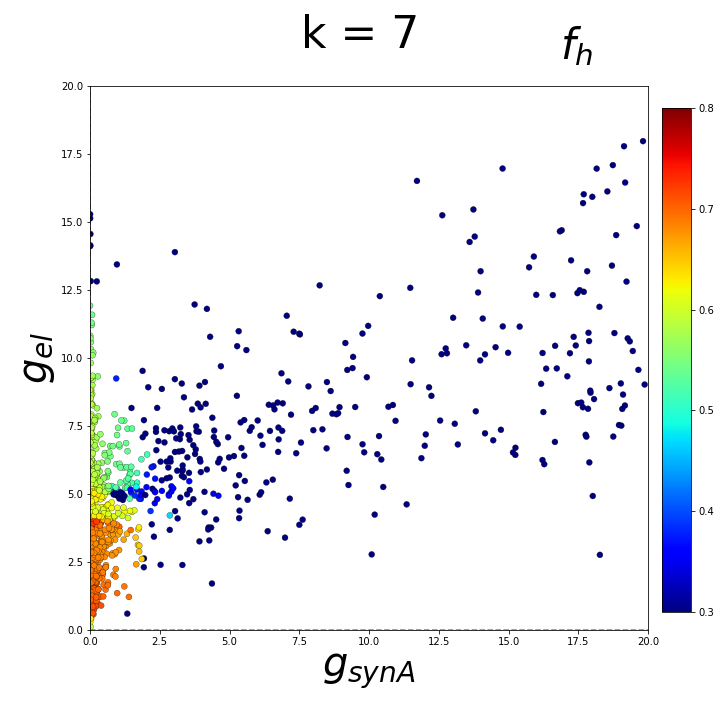
\includegraphics[scale=0.125]{DSN_figs/STGCircuit_DSN_c=0_rs=2_k=7.png}
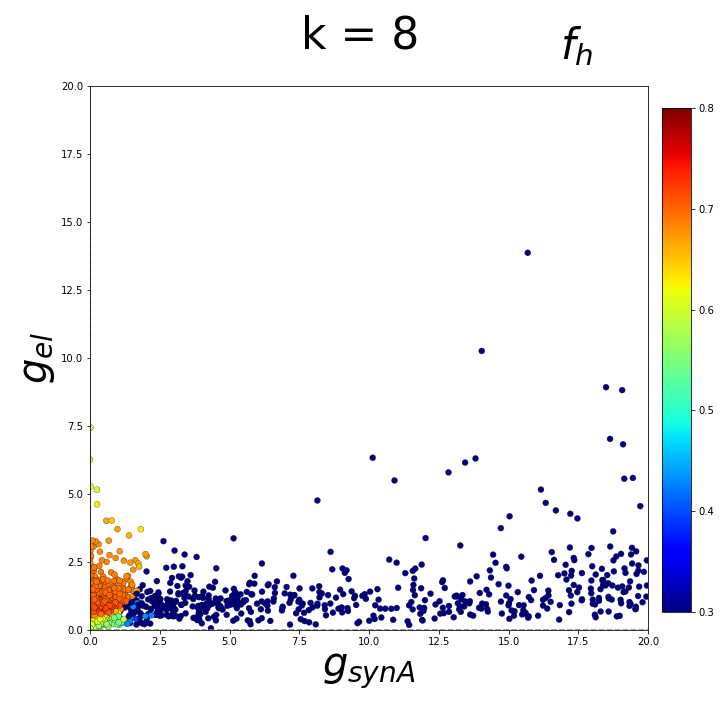
\includegraphics[scale=0.125]{DSN_figs/STGCircuit_DSN_c=0_rs=2_k=8.png}
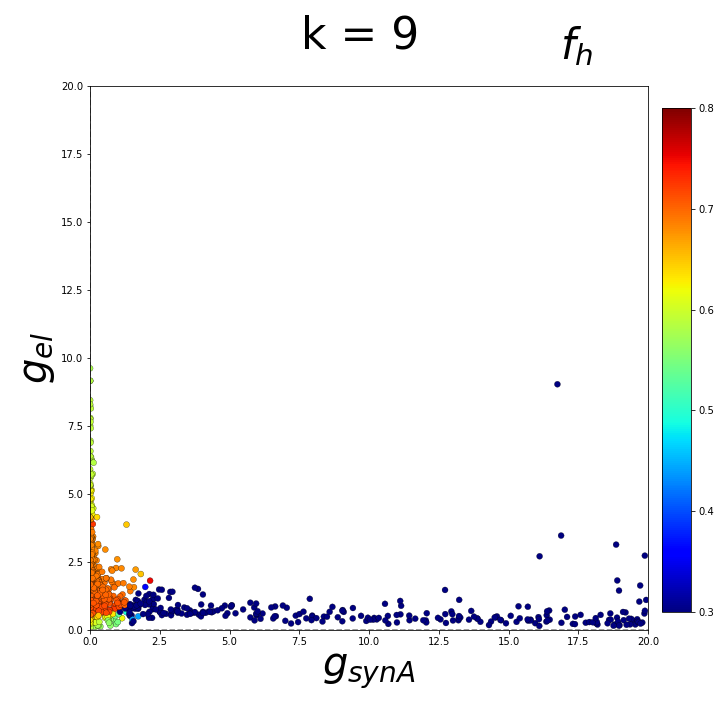
\includegraphics[scale=0.125]{DSN_figs/STGCircuit_DSN_c=0_rs=2_k=9.png}
\end{center}

\begin{center}
{\Large $c_0 = 1$, random seed = 3} \\
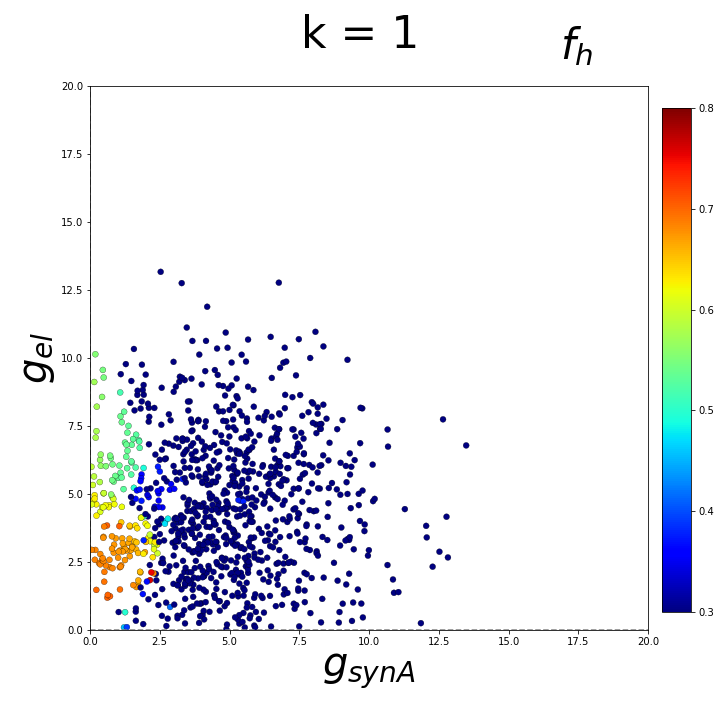
\includegraphics[scale=0.125]{DSN_figs/STGCircuit_DSN_c=0_rs=3_k=1.png}
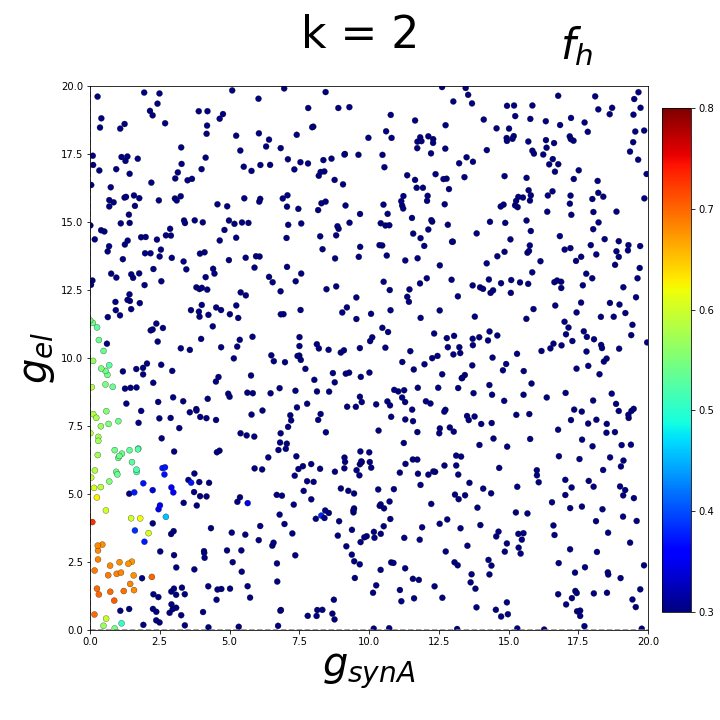
\includegraphics[scale=0.125]{DSN_figs/STGCircuit_DSN_c=0_rs=3_k=2.png}
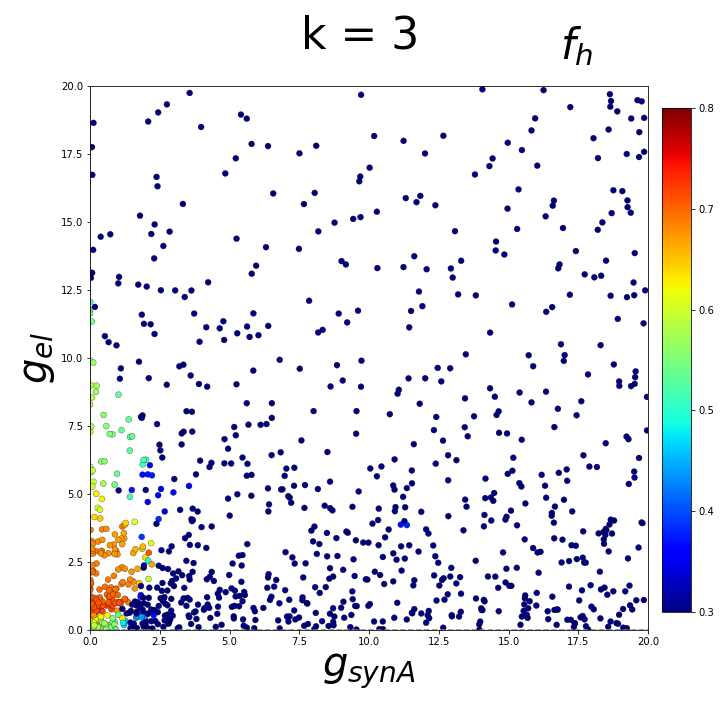
\includegraphics[scale=0.125]{DSN_figs/STGCircuit_DSN_c=0_rs=3_k=3.png}
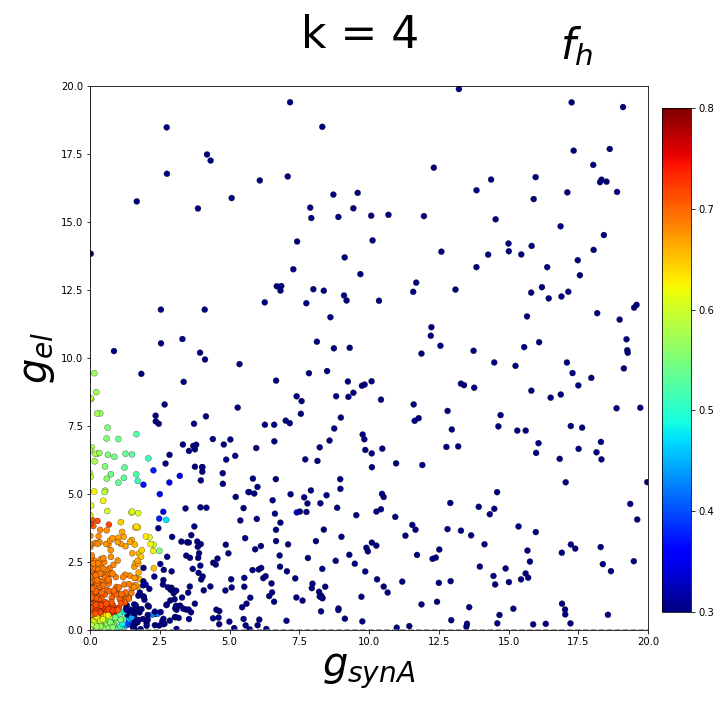
\includegraphics[scale=0.125]{DSN_figs/STGCircuit_DSN_c=0_rs=3_k=4.png}
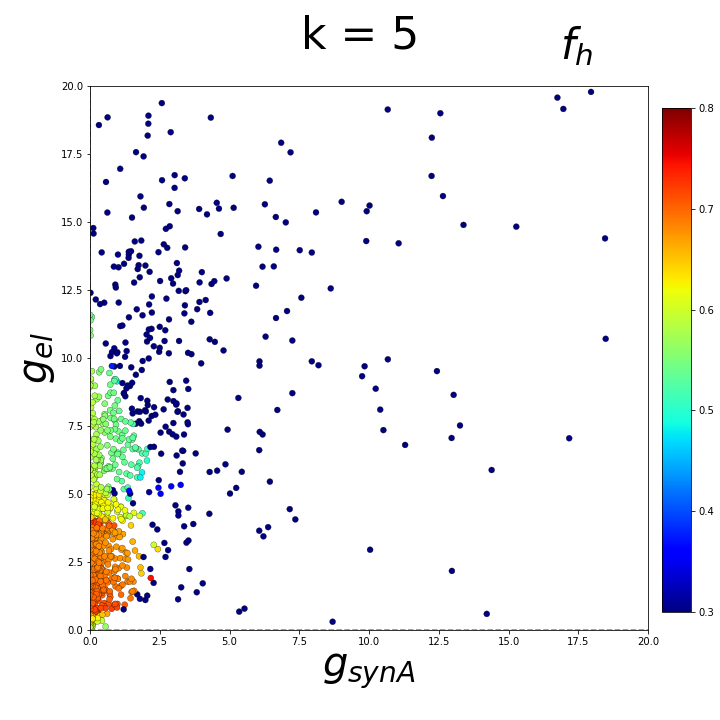
\includegraphics[scale=0.125]{DSN_figs/STGCircuit_DSN_c=0_rs=3_k=5.png}
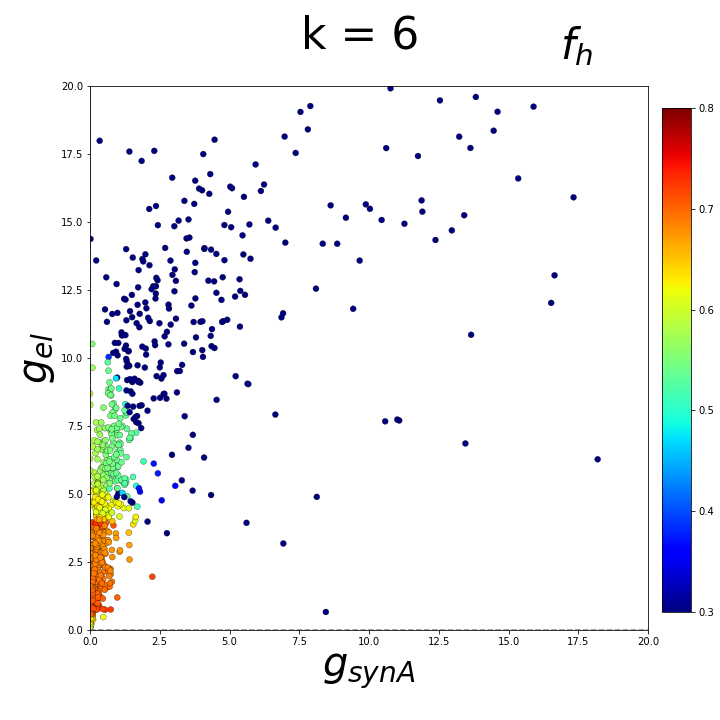
\includegraphics[scale=0.125]{DSN_figs/STGCircuit_DSN_c=0_rs=3_k=6.png}
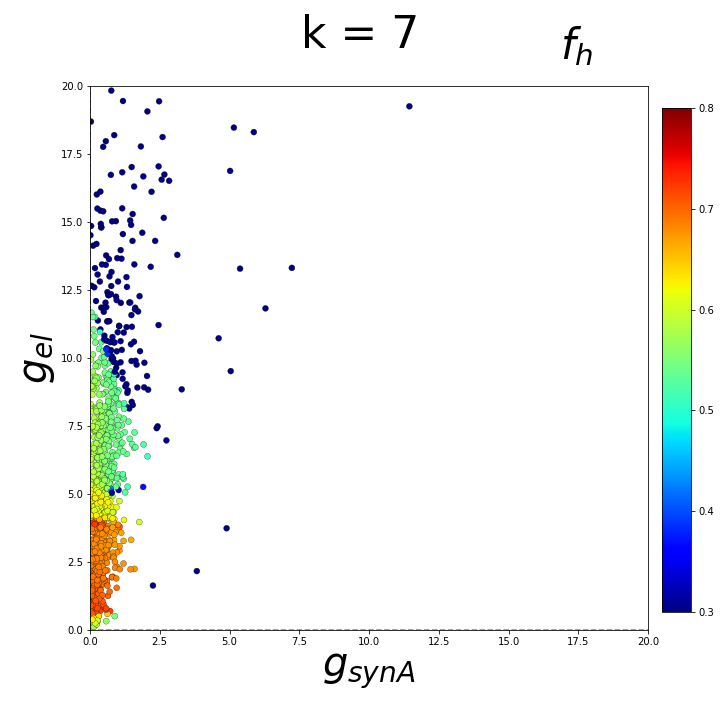
\includegraphics[scale=0.125]{DSN_figs/STGCircuit_DSN_c=0_rs=3_k=7.png}
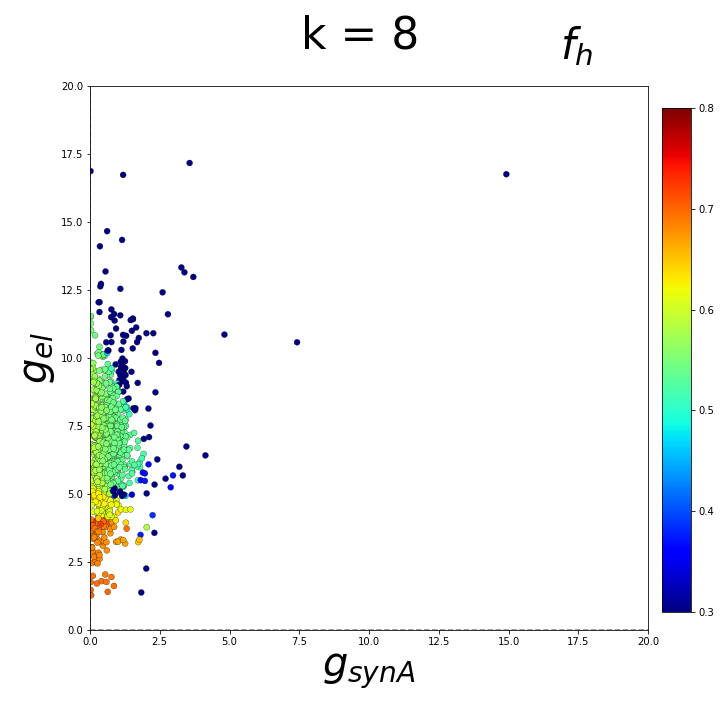
\includegraphics[scale=0.125]{DSN_figs/STGCircuit_DSN_c=0_rs=3_k=8.png}
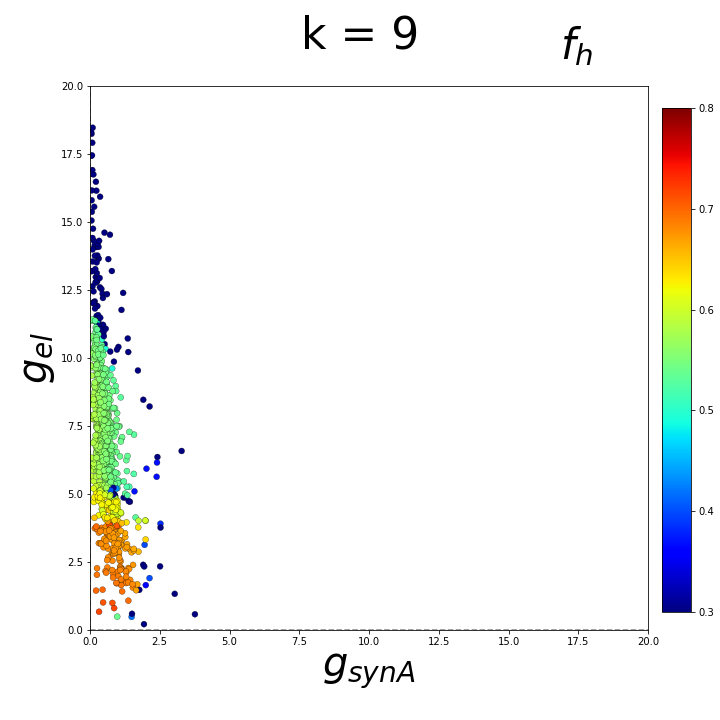
\includegraphics[scale=0.125]{DSN_figs/STGCircuit_DSN_c=0_rs=3_k=9.png}
\end{center}

\begin{center}
{\Large $c_0 = 1$, random seed = 4} \\
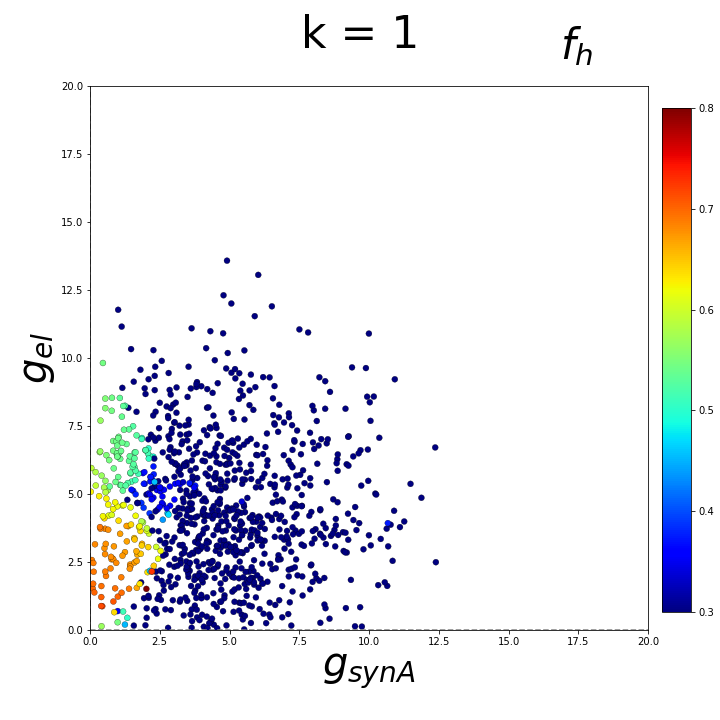
\includegraphics[scale=0.125]{DSN_figs/STGCircuit_DSN_c=0_rs=4_k=1.png}
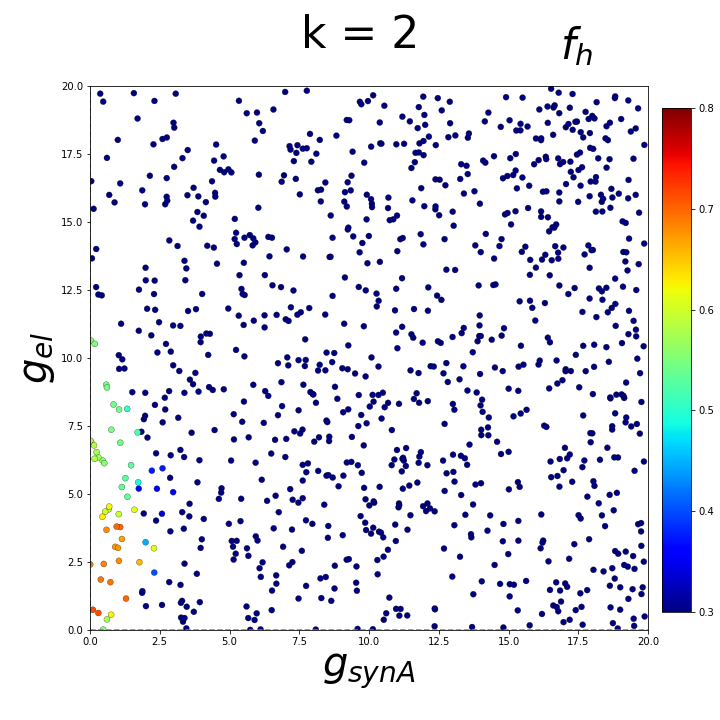
\includegraphics[scale=0.125]{DSN_figs/STGCircuit_DSN_c=0_rs=4_k=2.png}
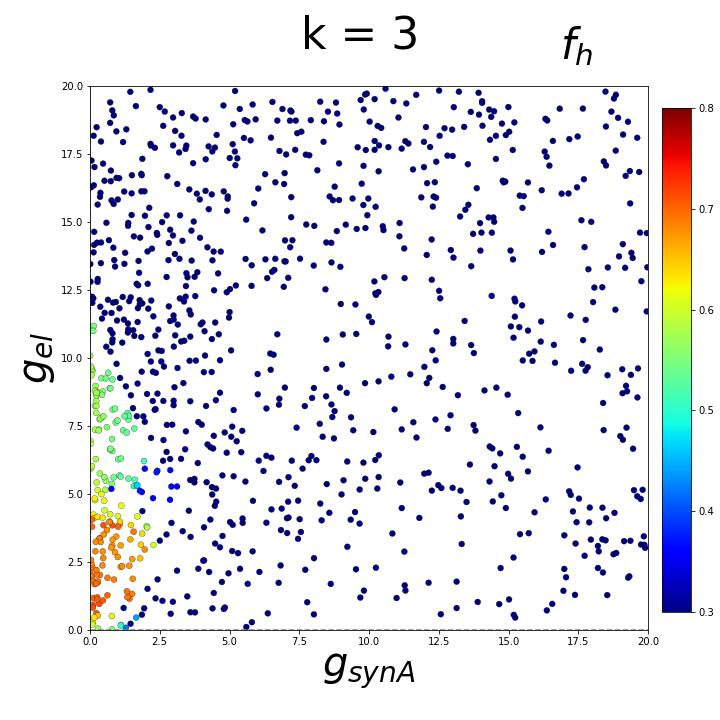
\includegraphics[scale=0.125]{DSN_figs/STGCircuit_DSN_c=0_rs=4_k=3.png}
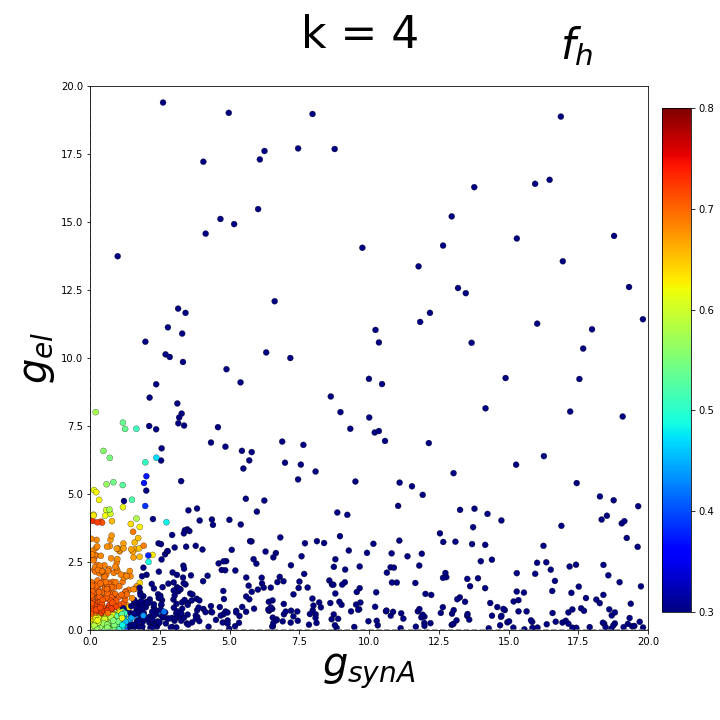
\includegraphics[scale=0.125]{DSN_figs/STGCircuit_DSN_c=0_rs=4_k=4.png}
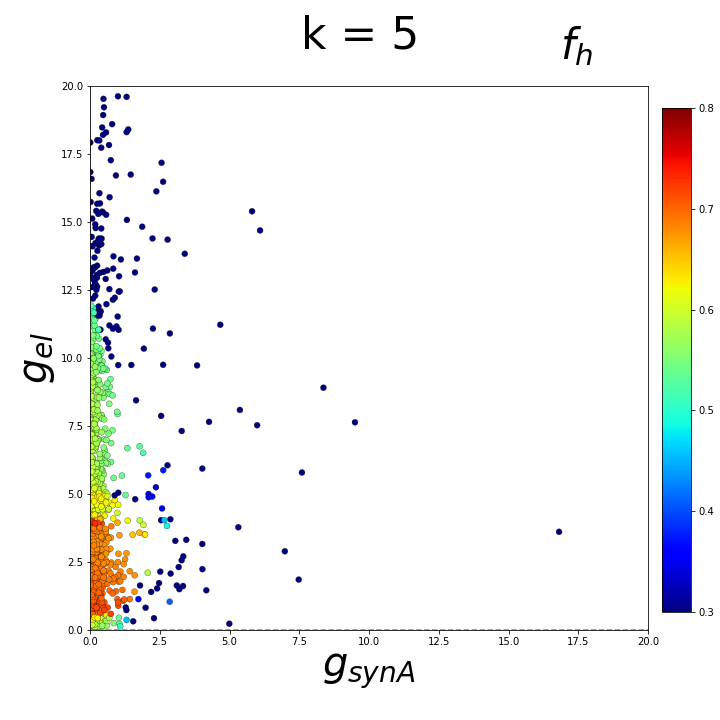
\includegraphics[scale=0.125]{DSN_figs/STGCircuit_DSN_c=0_rs=4_k=5.png}
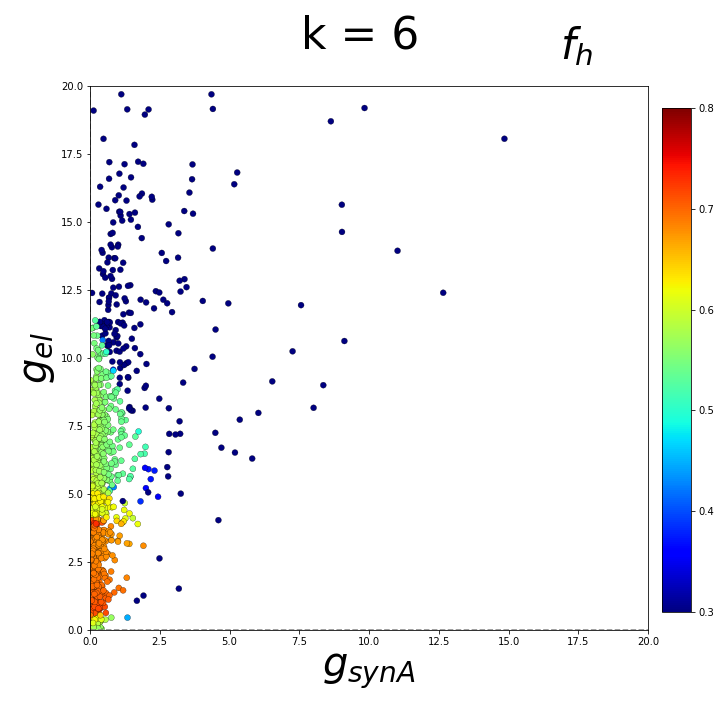
\includegraphics[scale=0.125]{DSN_figs/STGCircuit_DSN_c=0_rs=4_k=6.png}
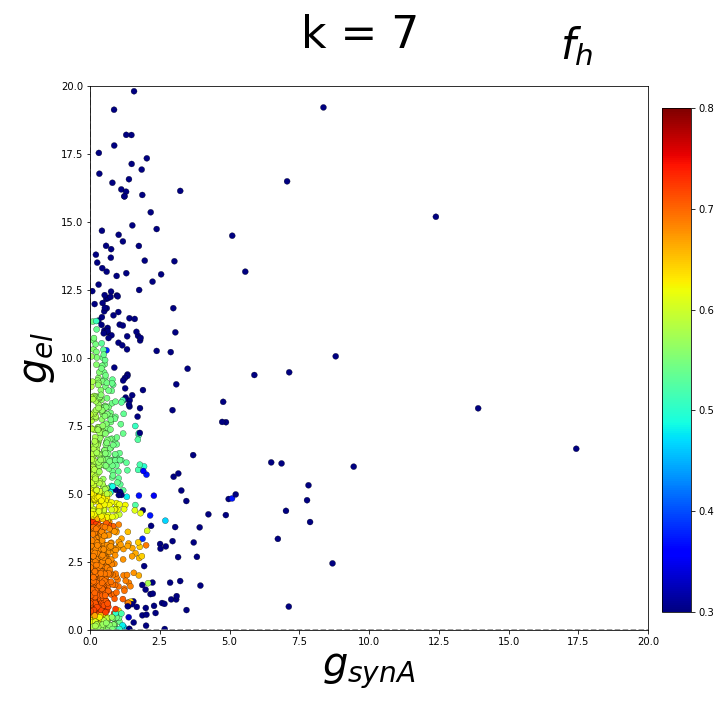
\includegraphics[scale=0.125]{DSN_figs/STGCircuit_DSN_c=0_rs=4_k=7.png}
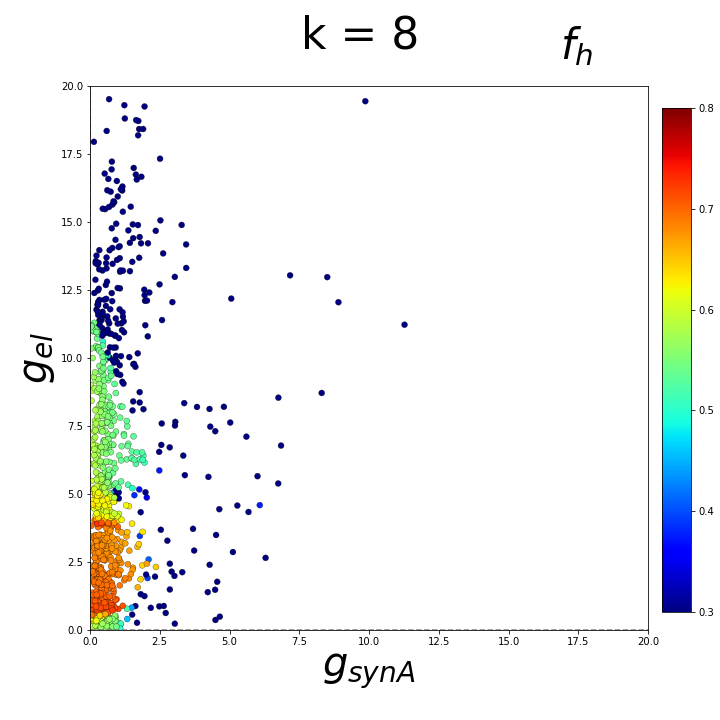
\includegraphics[scale=0.125]{DSN_figs/STGCircuit_DSN_c=0_rs=4_k=8.png}
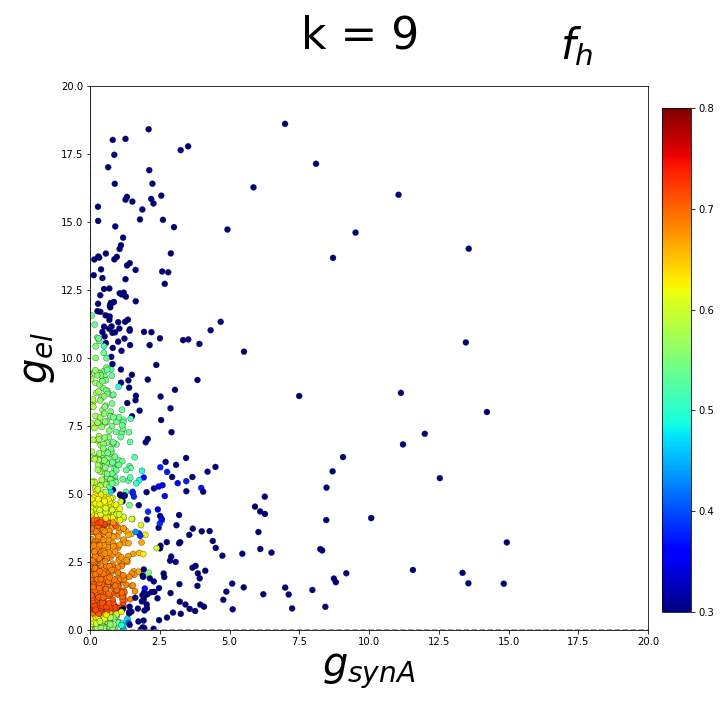
\includegraphics[scale=0.125]{DSN_figs/STGCircuit_DSN_c=0_rs=4_k=9.png}
\end{center}

\clearpage

\begin{center}
{\Large $c_0 = 100$} \\
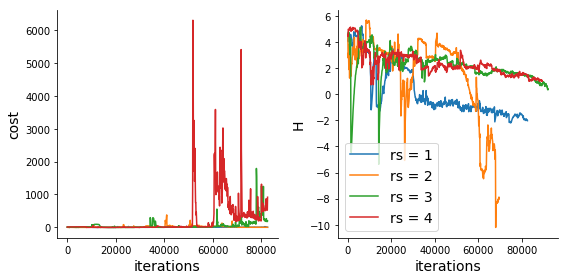
\includegraphics[scale=0.4]{DSN_figs/STG_DSN_c=2_H.png}
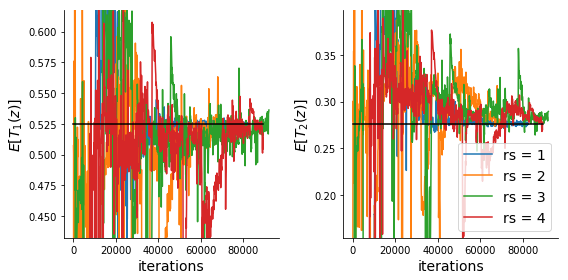
\includegraphics[scale=0.4]{DSN_figs/STG_DSN_c=2_cons.png} 
\end{center}

In contrast to $c_0 = 0$, we don't see an increase in entropy at the outset.  Two of these optimizations actually converge (rs=1, k=6 and rs=3, k=10), but to the individual lower and upper modes, respectively.

\begin{center}
{\Large $c_0 = 100$, random seed = 1} \\
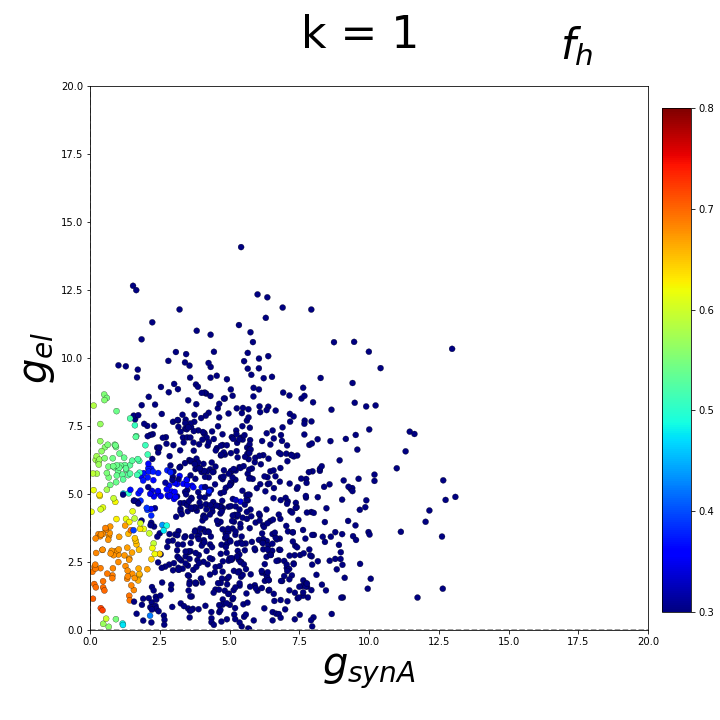
\includegraphics[scale=0.125]{DSN_figs/STGCircuit_DSN_c=2_rs=1_k=1.png}
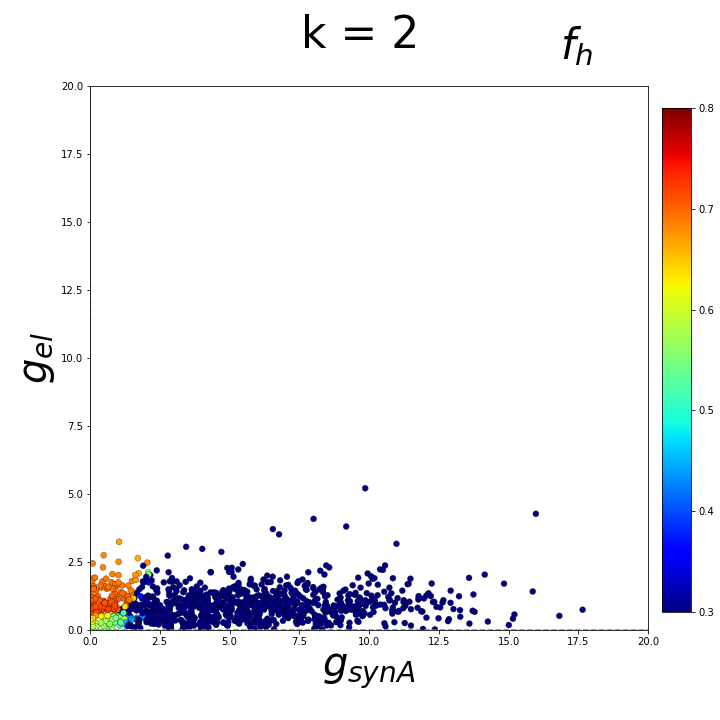
\includegraphics[scale=0.125]{DSN_figs/STGCircuit_DSN_c=2_rs=1_k=2.png}
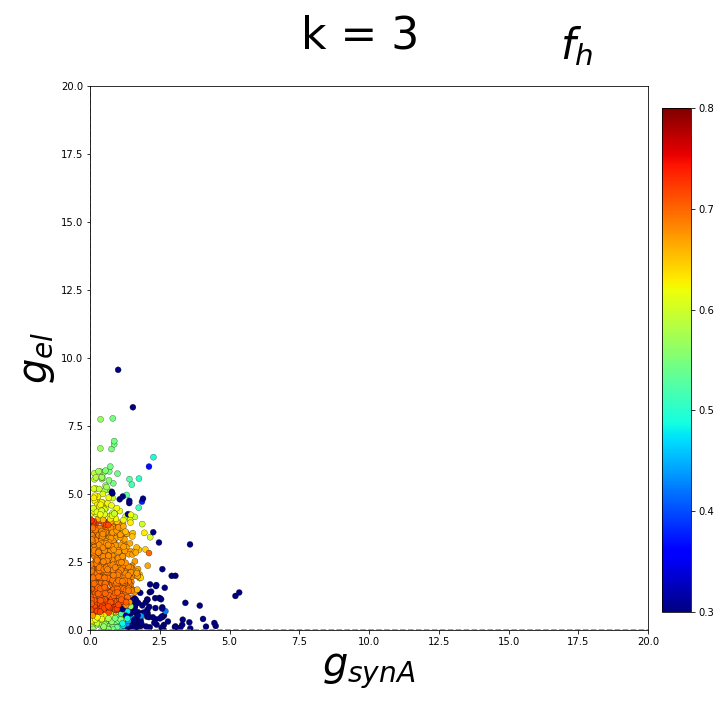
\includegraphics[scale=0.125]{DSN_figs/STGCircuit_DSN_c=2_rs=1_k=3.png}
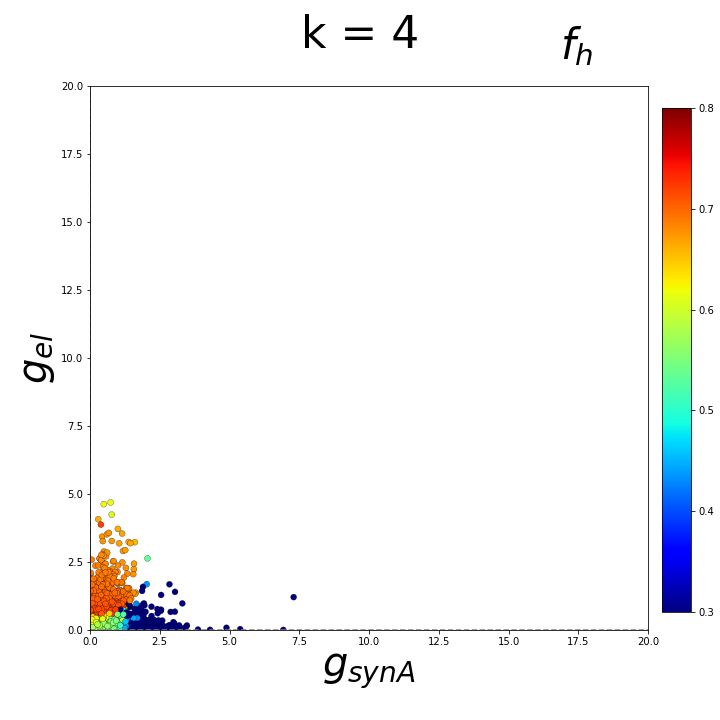
\includegraphics[scale=0.125]{DSN_figs/STGCircuit_DSN_c=2_rs=1_k=4.png}
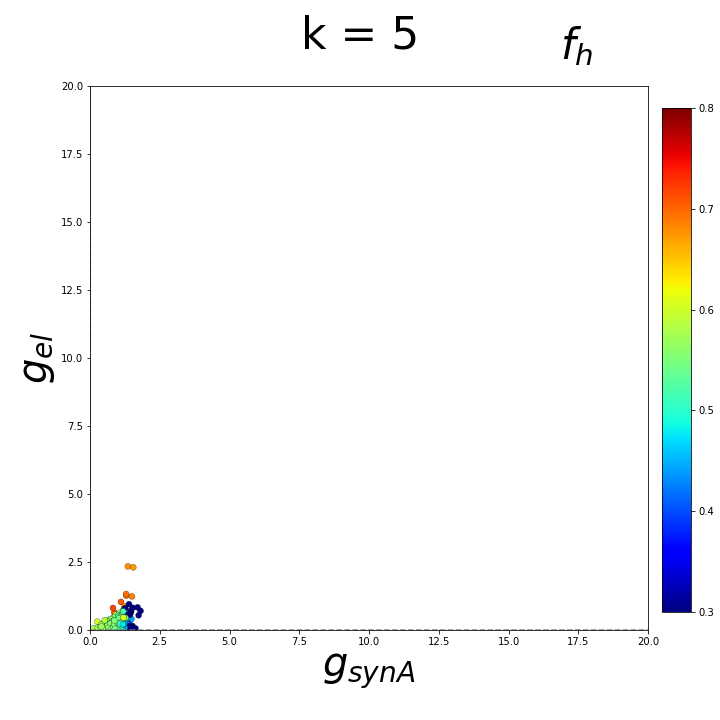
\includegraphics[scale=0.125]{DSN_figs/STGCircuit_DSN_c=2_rs=1_k=5.png} \\
{%
\setlength{\fboxsep}{0pt}%
\setlength{\fboxrule}{1pt}%
\fcolorbox{red}{white}{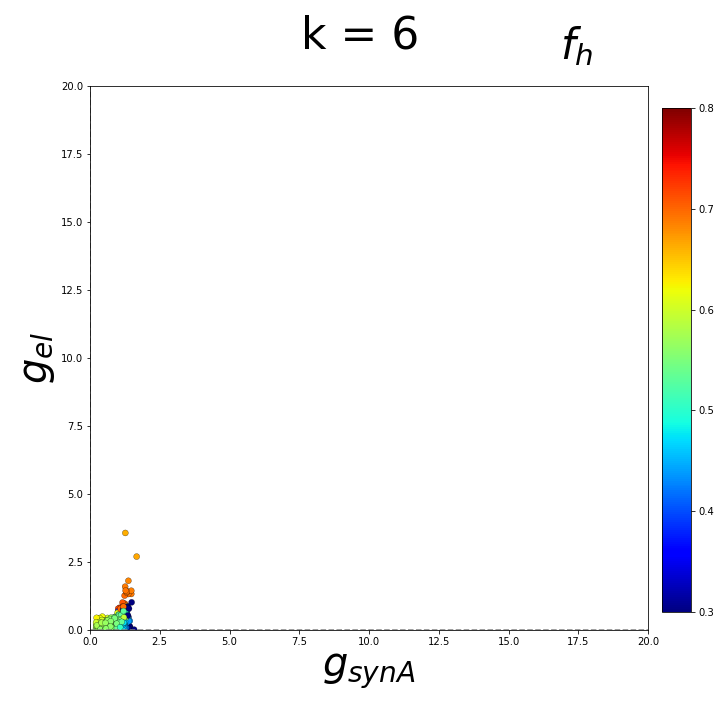
\includegraphics[scale=0.125]{DSN_figs/STGCircuit_DSN_c=2_rs=1_k=6.png}}%
}%
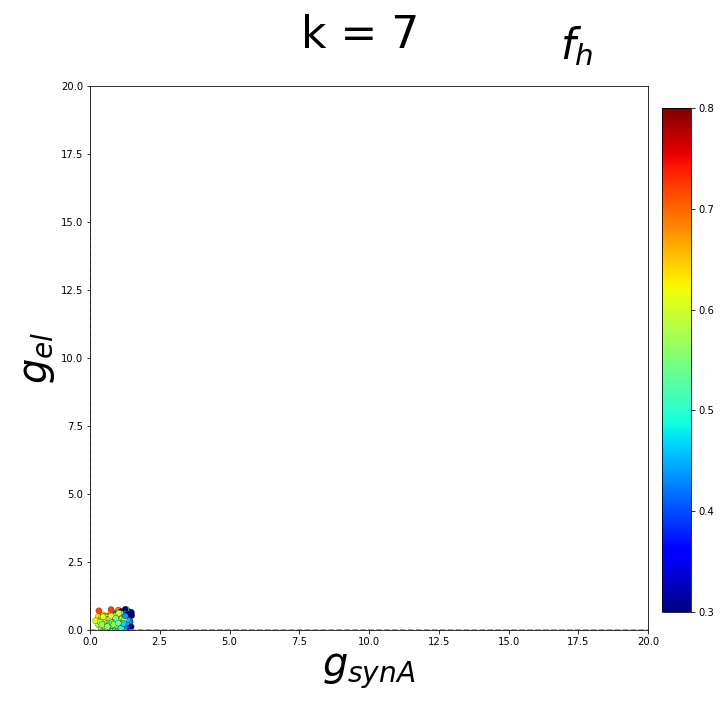
\includegraphics[scale=0.125]{DSN_figs/STGCircuit_DSN_c=2_rs=1_k=7.png}
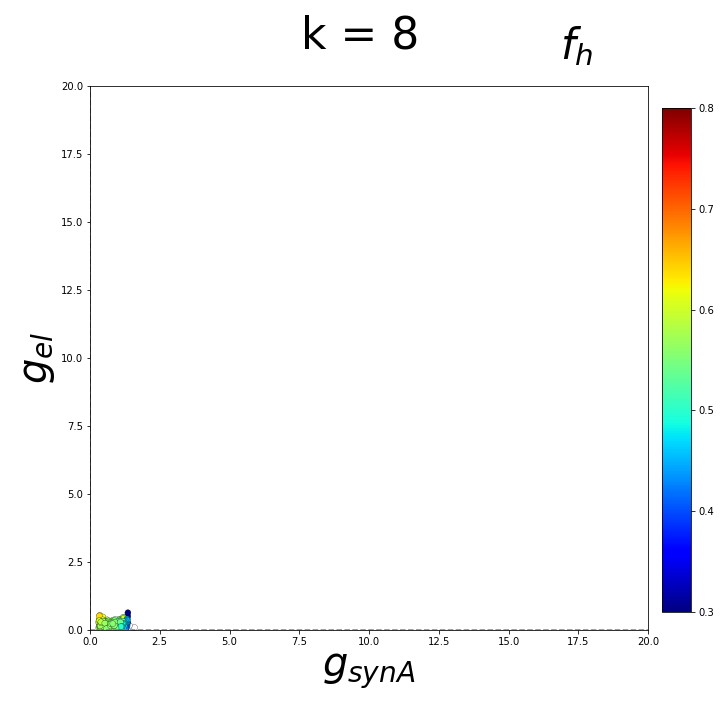
\includegraphics[scale=0.125]{DSN_figs/STGCircuit_DSN_c=2_rs=1_k=8.png}
\includegraphics[scale=0.125]{DSN_figs/STGCircuit_DSN_c=2_rs=1_k=9.png}
\end{center}


\begin{center}
{\Large $c_0 = 100$, random seed = 2} \\
\includegraphics[scale=0.125]{DSN_figs/STGCircuit_DSN_c=2_rs=2_k=1.png}
\includegraphics[scale=0.125]{DSN_figs/STGCircuit_DSN_c=2_rs=2_k=2.png}
\includegraphics[scale=0.125]{DSN_figs/STGCircuit_DSN_c=2_rs=2_k=3.png}
\includegraphics[scale=0.125]{DSN_figs/STGCircuit_DSN_c=2_rs=2_k=4.png}
\includegraphics[scale=0.125]{DSN_figs/STGCircuit_DSN_c=2_rs=2_k=5.png} \\
\includegraphics[scale=0.125]{DSN_figs/STGCircuit_DSN_c=2_rs=2_k=6.png}
\includegraphics[scale=0.125]{DSN_figs/STGCircuit_DSN_c=2_rs=2_k=7.png}
\end{center}

\begin{center}
{\Large $c_0 = 100$, random seed = 3} \\
\includegraphics[scale=0.125]{DSN_figs/STGCircuit_DSN_c=2_rs=3_k=1.png}
\includegraphics[scale=0.125]{DSN_figs/STGCircuit_DSN_c=2_rs=3_k=2.png}
\includegraphics[scale=0.125]{DSN_figs/STGCircuit_DSN_c=2_rs=3_k=3.png}
\includegraphics[scale=0.125]{DSN_figs/STGCircuit_DSN_c=2_rs=3_k=4.png}
\includegraphics[scale=0.125]{DSN_figs/STGCircuit_DSN_c=2_rs=3_k=5.png}
\includegraphics[scale=0.125]{DSN_figs/STGCircuit_DSN_c=2_rs=3_k=6.png}
\includegraphics[scale=0.125]{DSN_figs/STGCircuit_DSN_c=2_rs=3_k=7.png}
\includegraphics[scale=0.125]{DSN_figs/STGCircuit_DSN_c=2_rs=3_k=8.png}
\includegraphics[scale=0.125]{DSN_figs/STGCircuit_DSN_c=2_rs=3_k=9.png}
{%
\setlength{\fboxsep}{0pt}%
\setlength{\fboxrule}{1pt}%
\fcolorbox{red}{white}{\includegraphics[scale=0.125]{DSN_figs/STGCircuit_DSN_c=2_rs=3_k=10.png}}%
}%
\end{center}

\begin{center}
{\Large $c_0 = 100$, random seed = 4} \\
\includegraphics[scale=0.125]{DSN_figs/STGCircuit_DSN_c=2_rs=4_k=1.png}
\includegraphics[scale=0.125]{DSN_figs/STGCircuit_DSN_c=2_rs=4_k=2.png}
\includegraphics[scale=0.125]{DSN_figs/STGCircuit_DSN_c=2_rs=4_k=3.png}
\includegraphics[scale=0.125]{DSN_figs/STGCircuit_DSN_c=2_rs=4_k=4.png}
\includegraphics[scale=0.125]{DSN_figs/STGCircuit_DSN_c=2_rs=4_k=5.png}
\includegraphics[scale=0.125]{DSN_figs/STGCircuit_DSN_c=2_rs=4_k=6.png}
\includegraphics[scale=0.125]{DSN_figs/STGCircuit_DSN_c=2_rs=4_k=7.png}
\includegraphics[scale=0.125]{DSN_figs/STGCircuit_DSN_c=2_rs=4_k=8.png}
\includegraphics[scale=0.125]{DSN_figs/STGCircuit_DSN_c=2_rs=4_k=9.png}
\end{center}

\bibliography{dsn}
\bibliographystyle{unsrt}

\end{document}

